\section{Funcionamento}

\par O funcionamento do sistema organiza-se em camadas, conforme ilustrado na Figura~\ref{fig:arquitetura_sistema}. Essa organização separa responsabilidades entre a interface de supervisão, os serviços de domínio executados na nuvem, a persistência das informações e a conectividade com os equipamentos instalados.

\begin{figure}[H]
    \centering
    \caption{Arquitetura do Sistema}
    \centering
    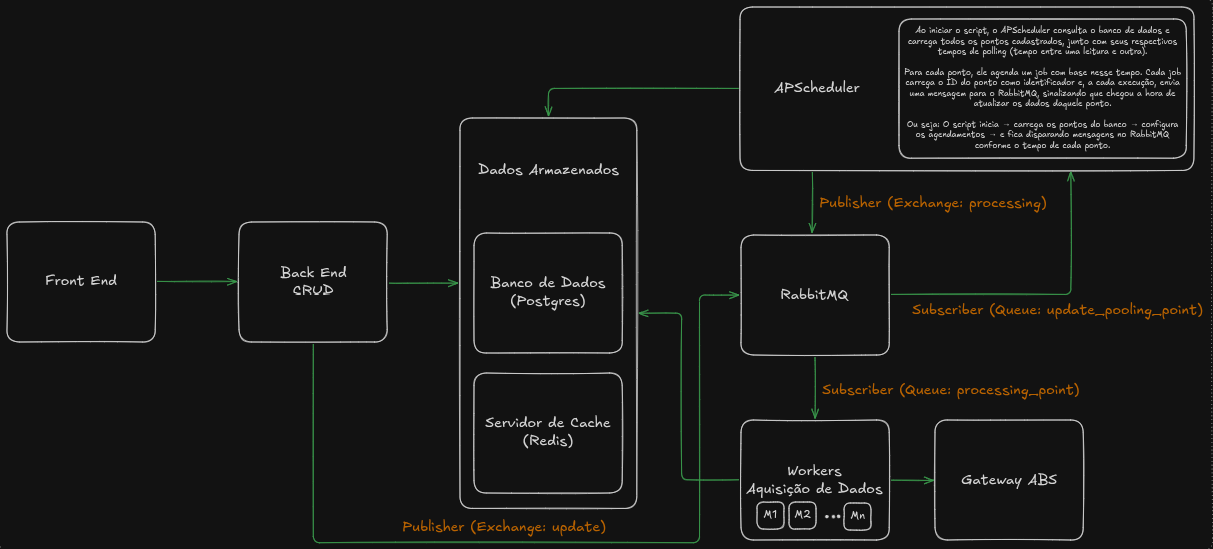
\includegraphics[width=0.9\textwidth]{Imagens/Desenvolvimento/Cap2/diagrama_servidores.png}
    \centering
    \vspace{0.2cm} \\
    Fonte: Autor.
    \label{fig:arquitetura_sistema}
\end{figure}

\par A Figura~\ref{fig:arquitetura_sistema} detalha a arquitetura completa do sistema. O \textbf{frontend} é desenvolvido em Next.js (Subseção~\ref{sec:nextjs}) e oferece a interface web de supervisão acessada pelos operadores em qualquer ponto da rede. O \textbf{backend CRUD} é construído em Fastify (Subseção~\ref{sec:fastify}) e expõe os \textit{endpoints} REST para cadastro de equipamentos, configuração de \emph{tags}, consulta de históricos e disparo de comandos. A camada de \textbf{dados armazenados} integra o banco relacional PostgreSQL, gerenciado pelo Amazon RDS (Subseções~\ref{sec:banco_dados} e~\ref{sec:aws}), com o servidor de cache Redis no Amazon ElastiCache (Subseção~\ref{sec:redis}), reunindo persistência histórica de longa duração e acesso de baixa latência ao estado corrente de cada \emph{tag}. O \textbf{APScheduler} é um servidor dedicado de agendamento que carrega no início da execução todos os pontos cadastrados no banco com seus respectivos tempos de \emph{polling} e, para cada ponto, agenda um \emph{job} próprio; a cada disparo, publica uma mensagem com o identificador do ponto, sinalizando que chegou a hora de atualizar aquele dado. O barramento entre os serviços é orquestrado pelo \textbf{Moleculer} (Subseção~\ref{sec:moleculer}), que recebe os comandos de aquisição no canal \texttt{processing} e os encaminha aos \textbf{workers de aquisição} (M1, M2, \ldots, Mn). Esses workers consumem o canal \texttt{processing\_point}, estabelecem sessão TCP com o \textit{Gateway ABS}, executam a leitura Modbus correspondente conforme tratado nas Subseções~\ref{sec:modbus_tcp_rtu} e~\ref{sec:m2m}, e devolvem o resultado ao barramento; o Moleculer então publica no canal \texttt{update} a leitura processada para que o banco persista o histórico e o cache atualize o valor corrente.

\subsection{Validações dos Requisitos do SCADA}
\label{sec:validacoes}

\par As subseções a seguir validam, item por item, o atendimento do sistema aos requisitos clássicos do SCADA descritos por \textcite{ZANGHI2019_SCADA_CONCEITOS} e revisados na Subseção~\ref{sec:scada}. Cada validação mostra como a arquitetura ilustrada na Figura~\ref{fig:arquitetura_sistema} e descrita acima atende aos seis pilares definidos: aquisição e registro de dados, sincronismo de tempo, níveis de acesso, comando e controle, escalabilidade e redundância.

\subsubsection{Aquisição e Registro de Dados}
\label{sec:req_aquisicao}

\par No quesito de aquisição e registro de dados discutido na Subseção~\ref{sec:scada}, o sistema atende a todos os requisitos descritos por \textcite{ZANGHI2019_SCADA_CONCEITOS}. A aquisição ocorre por meio dos workers, que se comunicam com IEDs e UTRs via Modbus pelo \textit{gateway} de borda e disponibilizam os valores em formato digital ao supervisório. Os pontos são cadastrados como \emph{tags} no banco de dados, classificadas como digitais (entrada DI, saída DO, memória DM) para representar estados binários como liga/desliga de motores e abertura/fechamento de válvulas, ou analógicas (entrada AI, saída AO, memória AM) para grandezas multibit como medições de pressão, vazão, nível e corrente. O registro contínuo das leituras na base de dados PostgreSQL sustenta as análises posteriores em gráficos de tendência e em relatórios sequenciais de eventos digitais, enquanto o cache Redis mantém os valores correntes acessíveis para a renderização imediata das telas de supervisão sem onerar o banco principal a cada atualização.

\subsubsection{Sincronismo de Tempo}
\label{sec:req_sincronismo}

\par O sincronismo de tempo exigido pelo SCADA é garantido pela combinação entre o relógio do APScheduler, sincronizado por NTP com a infraestrutura da AWS, e o carimbo de tempo aplicado pelos workers no instante exato em que a resposta Modbus é recebida do dispositivo de campo. Cada mensagem que trafega pelo barramento Moleculer carrega esse carimbo de tempo, que se preserva inalterado ao longo de toda a cadeia: do worker para o canal \texttt{update}, do canal para o banco e para o cache, do banco para o backend e do backend para o frontend. Assim, alarmes e eventos digitais captados em diferentes pontos do sistema recebem estampas de tempo coerentes na escala de milissegundos, atendendo à exigência de cronologia precisa para análises \emph{a posteriori} de ocorrências e faltas, sobretudo em processos com dinâmica rápida.

\subsubsection{Níveis de Acesso}
\label{sec:req_niveis}

\par No quesito de níveis de acesso discutido na Subseção~\ref{sec:scada}, o sistema substitui a hierarquia fixa de subestação por níveis de acesso definidos por planta. Cada usuário autentica-se no frontend Next.js e recebe uma sessão vinculada às instalações sob sua responsabilidade; o backend Fastify atua como ponto de autorização, validando, a cada requisição aos \textit{endpoints} REST, se o perfil do usuário permite consultar dados, configurar \emph{tags} ou disparar comandos da planta em questão. Dessa forma, a supervisão e o controle ficam segmentados conforme o cargo de cada operador, em consonância com o controle de acesso baseado em cargos e o princípio do menor privilégio \cite{STOUFFER2015_NIST_ICS_SECURITY}. Como a solução é multiplanta e compartilha a mesma infraestrutura na nuvem, esse isolamento de permissões por instalação é também uma medida de segurança, evitando que usuários de um cliente acessem ou comandem pontos de outro \cite{WALI2024_CLOUD_SCADA_SECURITY}.

\subsubsection{Comando e Controle}
\label{sec:req_comando}

\par O comando e controle previstos pelo SCADA são implementados nas três variantes descritas por \textcite{ZANGHI2019_SCADA_CONCEITOS}. O telecomando instantâneo, em que o operador no frontend dispara mudança imediata do estado de um equipamento (acionamento de bomba, abertura de válvula, comando a disjuntor), é traduzido em uma escrita Modbus pelo worker correspondente. O telecontrole, em que um \emph{set point} é definido pelo operador para regular no tempo a resposta de um processo, percorre o mesmo caminho mas atualiza um \textit{holding register} específico. O telecomando ou telecontrole programado, em que ações são agendadas conforme cenários previamente definidos, é mantido como configuração no banco e disparado pelo APScheduler no horário marcado, com o instante de execução registrado. As quatro fases do processamento (seleção, verificação, confirmação e execução) são distribuídas entre frontend (seleção e confirmação explícita por modal), backend Fastify (verificação de intertravamentos e condições de segurança) e worker (execução da escrita Modbus); após a execução, o próprio worker realiza uma leitura de verificação para confirmar que a solicitação foi aceita pelo dispositivo de campo, e, em caso de falha, gera o alarme correspondente para sinalizar a inconsistência ao operador.

\subsubsection{Escalabilidade}
\label{sec:req_escalabilidade}

\par A escalabilidade é atendida em três frentes complementares. Na expansão de cadastro, novos pontos e novas telas podem ser adicionados em produção sem alteração de código: o worker é parametrizado pelo banco (Subseção~\ref{sec:banco_dados}) e o frontend renderiza as telas dinamicamente conforme a configuração; o APScheduler reage à inclusão recarregando a lista de pontos e ajustando seus \emph{jobs}. Na capacidade de processamento, os workers (M1, M2, \ldots, Mn) podem ser replicados horizontalmente para distribuir a carga: o Moleculer faz balanceamento automático entre as instâncias que consomem o canal \texttt{processing\_point}, e o Amazon ECS (Subseção~\ref{sec:aws}) provisiona novas réplicas dos contêineres Docker conforme métricas de utilização. Na infraestrutura de dados, os serviços gerenciados Amazon RDS e ElastiCache escalam verticalmente sob demanda. Esse desenho elimina o gargalo de licenciamento por número de pontos típico de supervisórios comerciais e permite acompanhar a expansão das instalações sem reorçamento da solução, ainda que cuidados de capacidade dos elementos de rede e do barramento Moleculer devam ser considerados desde o projeto.

\subsubsection{Redundância}
\label{sec:req_redundancia}

\par A redundância acompanha a arquitetura em todas as camadas críticas, contemplando as recomendações de \textcite{ZANGHI2019_SCADA_CONCEITOS} e \textcite{SALVADOR2019_AQUISICAO_REDUNDANCIA}. Os workers de aquisição operam como uma frota em que cada instância consome trabalho de uma mesma fila gerenciada pelo Moleculer, de modo que a perda de um worker é absorvida pelos demais sem perda de leituras pendentes. O banco de dados em RDS é configurado com réplica em zona de disponibilidade distinta, com \emph{failover} automático em caso de falha do nó primário e \emph{snapshots} programados para recuperação ponto-a-ponto (Subseção~\ref{sec:banco_dados}). O cache Redis opera no modo \emph{cluster} com réplicas espelhadas (Subseção~\ref{sec:redis}). O frontend Next.js e o backend Fastify são executados em múltiplos contêineres atrás de um balanceador de carga, e o próprio barramento Moleculer pode ser configurado em \emph{cluster} para tolerância a falhas no transporte. Esse conjunto de medidas atinge níveis de confiabilidade compatíveis com a criticidade exigida em aplicações industriais sensíveis.

\subsection{Servidores}
\label{sec:servidores}

\par O sistema decompõe-se em sete componentes lógicos de servidor, cada qual com responsabilidade bem delimitada e ciclo de vida independente, em alinhamento com o paradigma de microsserviços discutido na Subseção~\ref{sec:microservicos} e defendido por \textcite{BIGHETI2020} para sistemas industriais orientados a serviços. Todos os componentes são empacotados como contêineres Docker (Subseção~\ref{sec:docker}) e orquestrados pelo Amazon ECS (Subseção~\ref{sec:aws}), o que permite implantação independente, escalabilidade granular e isolamento de dependências. Cada um dos sete servidores é descrito nas subseções a seguir quanto à tecnologia escolhida, à sua responsabilidade no sistema e às interfaces que mantém com os demais componentes.

\subsubsection{Frontend}
\label{sec:srv_frontend}

\par O servidor de frontend é desenvolvido em Next.js (Subseção~\ref{sec:nextjs}) e materializa a interface de supervisão acessada pelo operador via navegador. Suas telas incluem visualização de pontos ao vivo, dashboards de tendência histórica, cadastro de equipamentos e \emph{tags}, painéis de alarmes ativos e formulários administrativos. As telas de operação em tempo real adotam renderização no cliente com atualização incremental via WebSocket, garantindo latência baixa entre a leitura no campo e a apresentação ao operador; as telas de cadastro e relatórios adotam renderização no servidor (SSR), aproveitando o pré-processamento e a verificação de credenciais. A comunicação com o restante do sistema ocorre exclusivamente via APIs REST/JSON (Subseção~\ref{sec:http_rest_json}) e WebSocket, sem acoplamento direto com o banco ou com o barramento de eventos.

\subsubsection{Backend}
\label{sec:srv_backend}

\par O servidor de backend CRUD é construído sobre o \textit{framework} Fastify (Subseção~\ref{sec:fastify}) e expõe os \textit{endpoints} REST consumidos pelo frontend. Suas atribuições incluem operações de criação, leitura, atualização e remoção sobre o cadastro de clientes, unidades, equipamentos e \emph{tags}; consultas históricas com filtros de tempo, equipamento e ponto; gestão de usuários, perfis e permissões; e disparo de comandos de telecontrole pelo operador. Cada requisição é validada contra um esquema JSON Schema declarativo, autenticada por \emph{token} JWT armazenado no Redis e auditada em \textit{log} estruturado. Quando uma operação envolve interação com o campo (por exemplo, escrita Modbus), o backend não fala diretamente com os workers, mas publica um comando no barramento Moleculer, mantendo o desacoplamento entre a camada de aplicação e a camada de aquisição.

\subsubsection{Banco de Dados}
\label{sec:srv_banco_dados}

\par O servidor de banco de dados é uma instância PostgreSQL gerenciada pelo Amazon RDS (Subseções~\ref{sec:banco_dados} e~\ref{sec:aws}), responsável pela persistência de longa duração de todo o estado relevante do sistema: cadastro hierárquico (cliente, unidade operacional, equipamento, \emph{tag}), histórico de leituras com carimbo de tempo, eventos de alarme, registros de auditoria, configuração de usuários e parâmetros de comunicação. O esquema relacional aproveita chaves estrangeiras para garantir integridade referencial; tabelas históricas são particionadas por intervalo de tempo para evitar tabelas monolíticas, e índices nos campos \texttt{tag\_id} e \texttt{timestamp} aceleram as consultas mais frequentes. A configuração em produção emprega réplica em zona de disponibilidade distinta, com \emph{failover} automático em caso de falha do nó primário e \emph{snapshots} programados para recuperação ponto-a-ponto, conforme recomendado por \textcite{SALVADOR2019_AQUISICAO_REDUNDANCIA}.

\subsubsection{Cache}
\label{sec:srv_cache}

\par O servidor de cache é uma instância Redis provida pelo Amazon ElastiCache (Subseção~\ref{sec:redis}) e cumpre três papéis simultâneos. Como cache de leituras frequentes, mantém em memória o valor corrente de cada \emph{tag} ativa, acessado pelas telas de supervisão em tempo real sem onerar o banco principal a cada atualização. Como barramento publicador-assinante de baixa latência, distribui eventos de aquisição aos consumidores interessados (alarmes, históricos, frontend ao vivo). Como armazenamento efêmero, abriga \textit{tokens} de autenticação, contadores de limitação de requisições por usuário (\emph{rate limiting}) e travas distribuídas que evitam processamento duplicado de comandos críticos. O cluster opera com réplicas espelhadas em zonas distintas e expiração automática (TTL) das chaves voláteis.

\subsubsection{APScheduler}
\label{sec:srv_apscheduler}

\par O servidor de agendamento executa a biblioteca APScheduler em um contêiner dedicado e é responsável por decidir o instante em que cada ponto deve ser lido. No início da execução, o serviço consulta o banco de dados, carrega todos os pontos cadastrados com seus respectivos tempos de \emph{polling} (intervalo entre uma leitura e a próxima) e agenda um \emph{job} próprio para cada ponto com base nesse tempo. A cada disparo, o \emph{job} carrega o identificador do ponto e publica uma mensagem no barramento Moleculer, sinalizando aos workers que chegou a hora de atualizar aquele dado. O servidor reage a mudanças no cadastro (inclusão, remoção ou alteração de periodicidade) por meio de mecanismo de invalidação que recarrega os \emph{jobs} afetados, sem necessidade de reinício; janelas de manutenção e leituras prioritárias também são tratadas nessa camada, separando a decisão ``quando ler'' da execução ``como ler''.

\subsubsection{Barramento Moleculer}
\label{sec:srv_moleculer}

\par O servidor de barramento de mensagens é uma instância do Moleculer (Subseção~\ref{sec:moleculer}) que orquestra a comunicação assíncrona entre os demais componentes. Três canais principais estruturam o tráfego: o canal \texttt{processing} recebe comandos de aquisição emitidos pelo APScheduler e pelo backend (no caso de leituras sob demanda); o canal \texttt{processing\_point} é consumido pelos workers de aquisição em modo de balanceamento de carga; e o canal \texttt{update} carrega os resultados das leituras de volta para o banco e para o cache, além de servir como gatilho para os serviços de alarmes e de notificação. O Moleculer também fornece descoberta automática de serviços, balanceamento entre instâncias replicadas, \emph{circuit breakers} para isolamento de falhas em cascata e \emph{distributed tracing} para rastreabilidade fim a fim das requisições que atravessam vários serviços.

\subsubsection{Workers de Aquisição}
\label{sec:srv_workers}

\par Os workers de aquisição (M1, M2, \ldots, Mn) constituem a frota responsável pela comunicação efetiva com o campo. Cada worker é uma instância idêntica de um contêiner Docker, replicável horizontalmente conforme a carga, e mantém um conjunto de sessões TCP ativas com os \textit{gateways} ABS de cada cliente. Ao consumir uma mensagem do canal \texttt{processing\_point}, o worker monta o telegrama Modbus correspondente (com base nos parâmetros do ponto recuperados do cadastro), envia a requisição pelo \textit{gateway}, valida a resposta, aplica a conversão para unidade de engenharia descrita na Subseção~\ref{sec:escala_engenharia} e publica o resultado no canal \texttt{update}. Os workers são \textit{stateless}, o que viabiliza adição ou remoção de instâncias sem perda de estado; políticas de \emph{timeout}, retentativa e \emph{backoff} exponencial são parametrizadas por equipamento, mantendo a robustez frente a falhas transitórias de comunicação.

\subsection{Aquisição de Dados}

\par A camada de aquisição de dados é o subsistema responsável por traduzir o estado físico do processo (níveis, vazões, pressões, energia, status de bombas e válvulas, alarmes, contadores etc.) em valores digitais confiáveis, com referência temporal e com metadados suficientes para consumo pela supervisão, por relatórios operacionais e por rotinas de histórico. Em termos práticos, ela engloba desde a montagem das requisições até a entrega dos dados já convertidos para unidades de engenharia (valores nas unidades físicas usuais na operação, como metro, m$^3$/h, bar ou kW). Com frequência, o equipamento expõe a grandeza apenas como inteiro em um ou mais registradores Modbus; o programa do CLP grava então uma representação em ponto fixo (por exemplo, o nível em centímetros com uma casa decimal vem como inteiro que deve ser dividido por 10, ou a vazão usa divisor 100), e cabe à camada de aquisição aplicar a multiplicação ou divisão, somas de deslocamento (\textit{offset}) e demais fatores de escala cadastrados para reproduzir o valor real usado na operação, prontos para gravação em banco.

\par Por operar em ambiente de nuvem, a arquitetura prevê um ponto de concentração na borda da solução (o \textit{gateway}) e dispositivos de campo (os modems), que mantêm a sessão com a infraestrutura central e encaminham o tráfego até o equipamento industrial conectado localmente, via serial RS-485 ou Ethernet. O \textit{gateway} recebe múltiplas conexões TCP vindas dos serviços na nuvem e, com base em regras de roteamento, direciona cada fluxo ao modem associado a um ponto remoto. O modem, por sua vez, materializa o enlace de longa distância (GPRS ou outro meio de acesso à internet) e encerra a parte WAN da comunicação, entregando ao equipamento final a mensagem no formato esperado.

\par Na prática, é comum encontrar soluções integradas por fornecedores de telemetria, a título de exemplificação, o \textit{gateway} ABS (Figura~\ref{fig:gateway_abs}) e o modem GPRS ABS Cel X (Figura~\ref{fig:modem_gprs}) representam a camada física de conectividade adotada em muitos projetos: o primeiro agrega e roteia sessões, o segundo viabiliza o acesso móvel em um ponto de medição remoto.

\begin{figure}[H]
    \centering
    \caption{Gateway ABS}
    \centering
    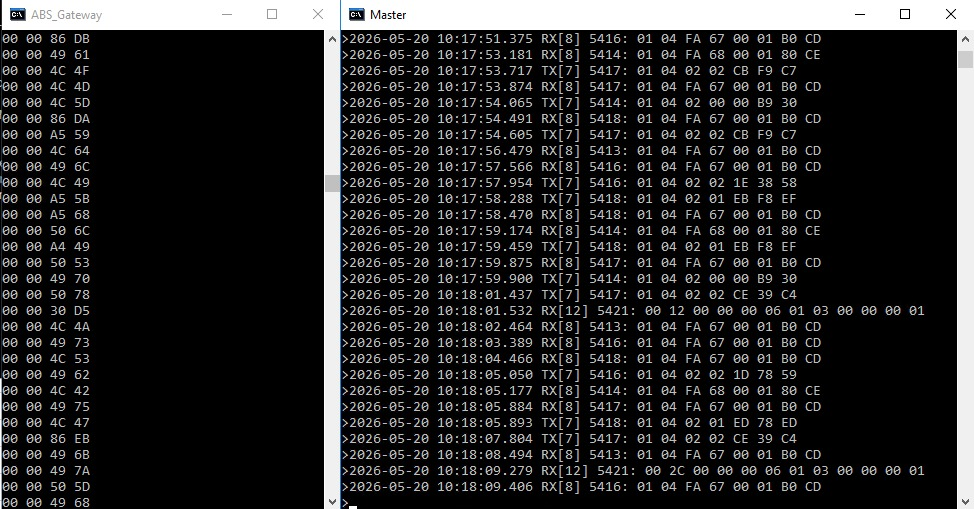
\includegraphics[width=0.9\textwidth]{Imagens/Desenvolvimento/Cap2/gateway_abs.jpeg}
    \centering
    \vspace{0.2cm} \\
    Fonte: Autor.
    \label{fig:gateway_abs}
\end{figure}

\begin{figure}[H]
    \centering
    \caption{Modem GPRS ABS Cel X}
    \centering
    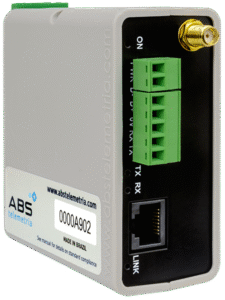
\includegraphics[width=0.9\textwidth]{Imagens/Desenvolvimento/Cap2/cel_x.png}
    \centering
    \vspace{0.2cm} \\
    Fonte: Autor.
    \label{fig:modem_gprs}
\end{figure}



\par Entre a nuvem e o equipamento de campo, o protocolo de aplicação adotado para leitura e escrita das variáveis de processo é o Modbus. O encadeamento completo (serviço de aquisição, \textit{gateway}, modem e dispositivo escravo) preserva a semântica das funções Modbus (códigos de função, endereços de registradores ou \textit{coils}, dados de resposta), variando apenas o ``envelope'' de transporte: quadros TCP/IP na WAN e, no trecho serial, quadro RTU com verificação por CRC. O modo TCP e o modo RTU, bem como o encapsulamento usual em arquiteturas com telemetria, são tratados na Subseção~\ref{sec:modbus_tcp_rtu}.

